\section{Simplified architecture}
\textit{Figure \ref{fig:simplified_architecture}} shows a complete view of the entities composing the simplified architecture for the Interconnected project (that can be compared to the full architecture shown in \textit{figure \ref{fig:architecture_complete}}).

\begin{figure}[!ht]
    \centering
    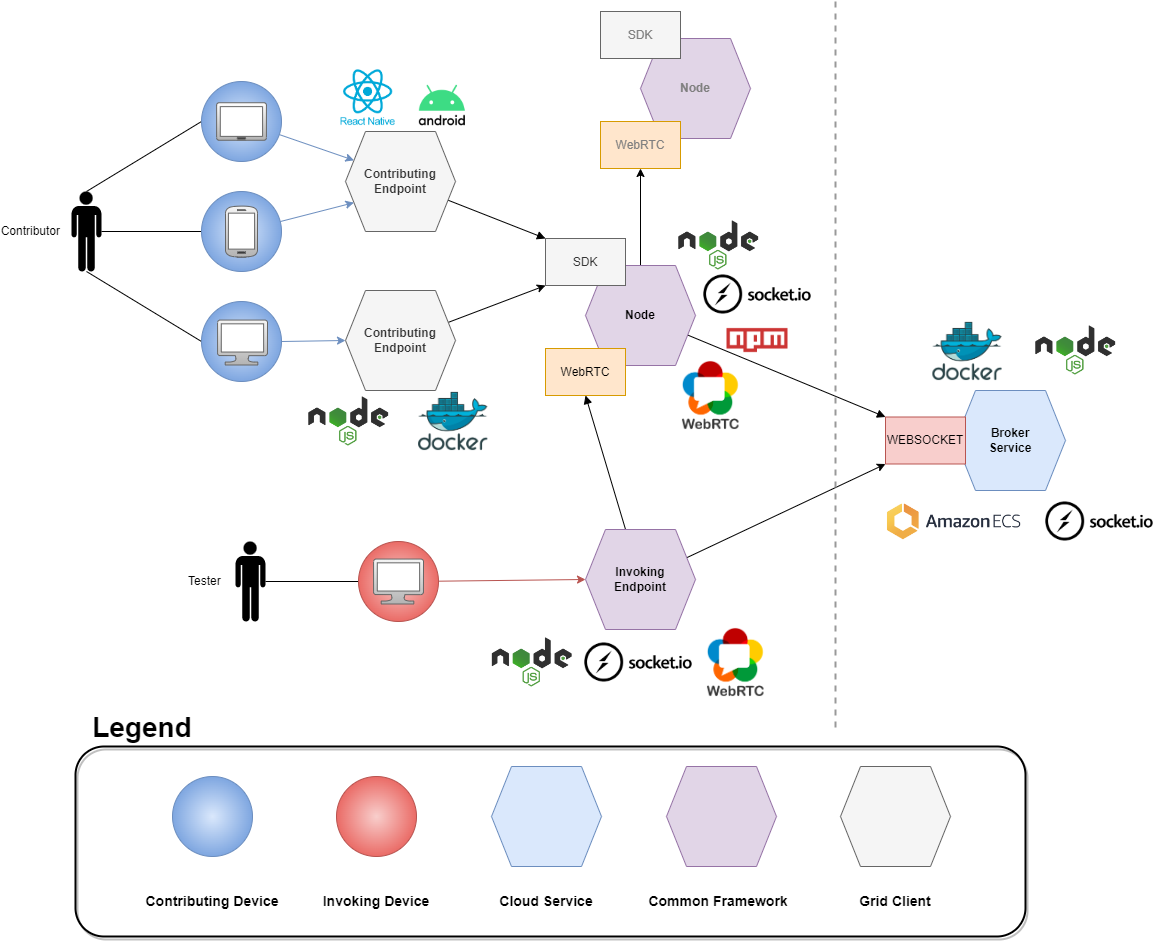
\includegraphics[width=\linewidth]{document/chapters/chapter_7/images/simplified_architecture.png}
    \caption{Complete view of the simplified prototype's architecture}
    \label{fig:simplified_architecture}
\end{figure}

\vspace{10mm}

All the entities composing the architecture are implemented using technologies based on Node.js which offers useful, popular and well maintained frameworks as well as an easy to use concurrency model based on an event loop.

\subsection{Broker Service}
The only Cloud Service present in this simplified architecture is the Broker Service; since only one instance (with a static address) of such Cloud Service is required to sustain the workload of the few devices connected, a dynamic handling and discovery of multiple instances is thus not required. As a direct consequence of that, the complementary entities that handled the dynamic system for scalability (Grid Master Service, Broker Discovery Service and Grid Services Gateway Service) are not needed and thus Nodes and Invoking Endpoints communicate directly with the Broker Service without first undergoing the discovery processes described in \textit{section \ref{use_cases_satisfaction}}.

The prototype's Broker Service is implemented by using the Typescript language and utilizes Socket.io in order to create a web server that is reachable via WebSocket protocol; through the use of this technology, Invoking Endpoints are able to deposit requests for the recruitment of Nodes that will be used to perform computations. The messages involved in the recruiting process and the general Grid connection will be discussed in \textit{section \ref{coordination}}.

In order to have a running instance of the Broker Service that also has a static address reachable from anywhere, a Docker image is created which, in turn, is executed in a container through the use of Amazon ECS (Elastic Container Service). More details about the deployment of this entity will be discussed later in \textit{section \ref{devops}}.

\subsection{Interconnected Node}
TODO technologies and stuff

The Node entity concretizes its P2P connectivity requirements through the use of the WebRTC (Real-Time Communication for the Web) protocol; such communication standard it is used to send audio and video data among peers, as well as any kind of structured non-media data. In order for the peers to establish the connection, first the signaling process needs to be completed: the peers, through a third intermediary (the Broker Service), exchange some information required for the connection to happen; the Peer that initializes the connection creates an SDP (Signaling Description Protocol) object, denominated "offer". When the other Peer receives such data, it also creates its SDP object denominated "answer". Once each Peers posses both generated SDP data, they finalize the connection exchanging some ICE (Interactive Connectivity Establishment) candidates; such ICE candidates needs to be specified when realizing a WebRTC connection since they are the actual servers that allow the P2P connection. There are two types of servers involved:
\begin{itemize}
    \item \textbf{STUN} (Session Traversal Utilities for NAT)\\
    Used by Peers that resides behind the same NAT; through this server the IP info of each Peer are retrieved and a direct P2P connection can be established.
    \item \textbf{TURN} (Traversal Using Relays around NAT)\\
    Used by Peers that resides in different NATs; through this server the limitations of a NAT are overcome, creating an indirect P2P connection that uses the TURN server to forward the messages among the two Peers.
\end{itemize}

\begin{figure}[!ht]
    \centering
    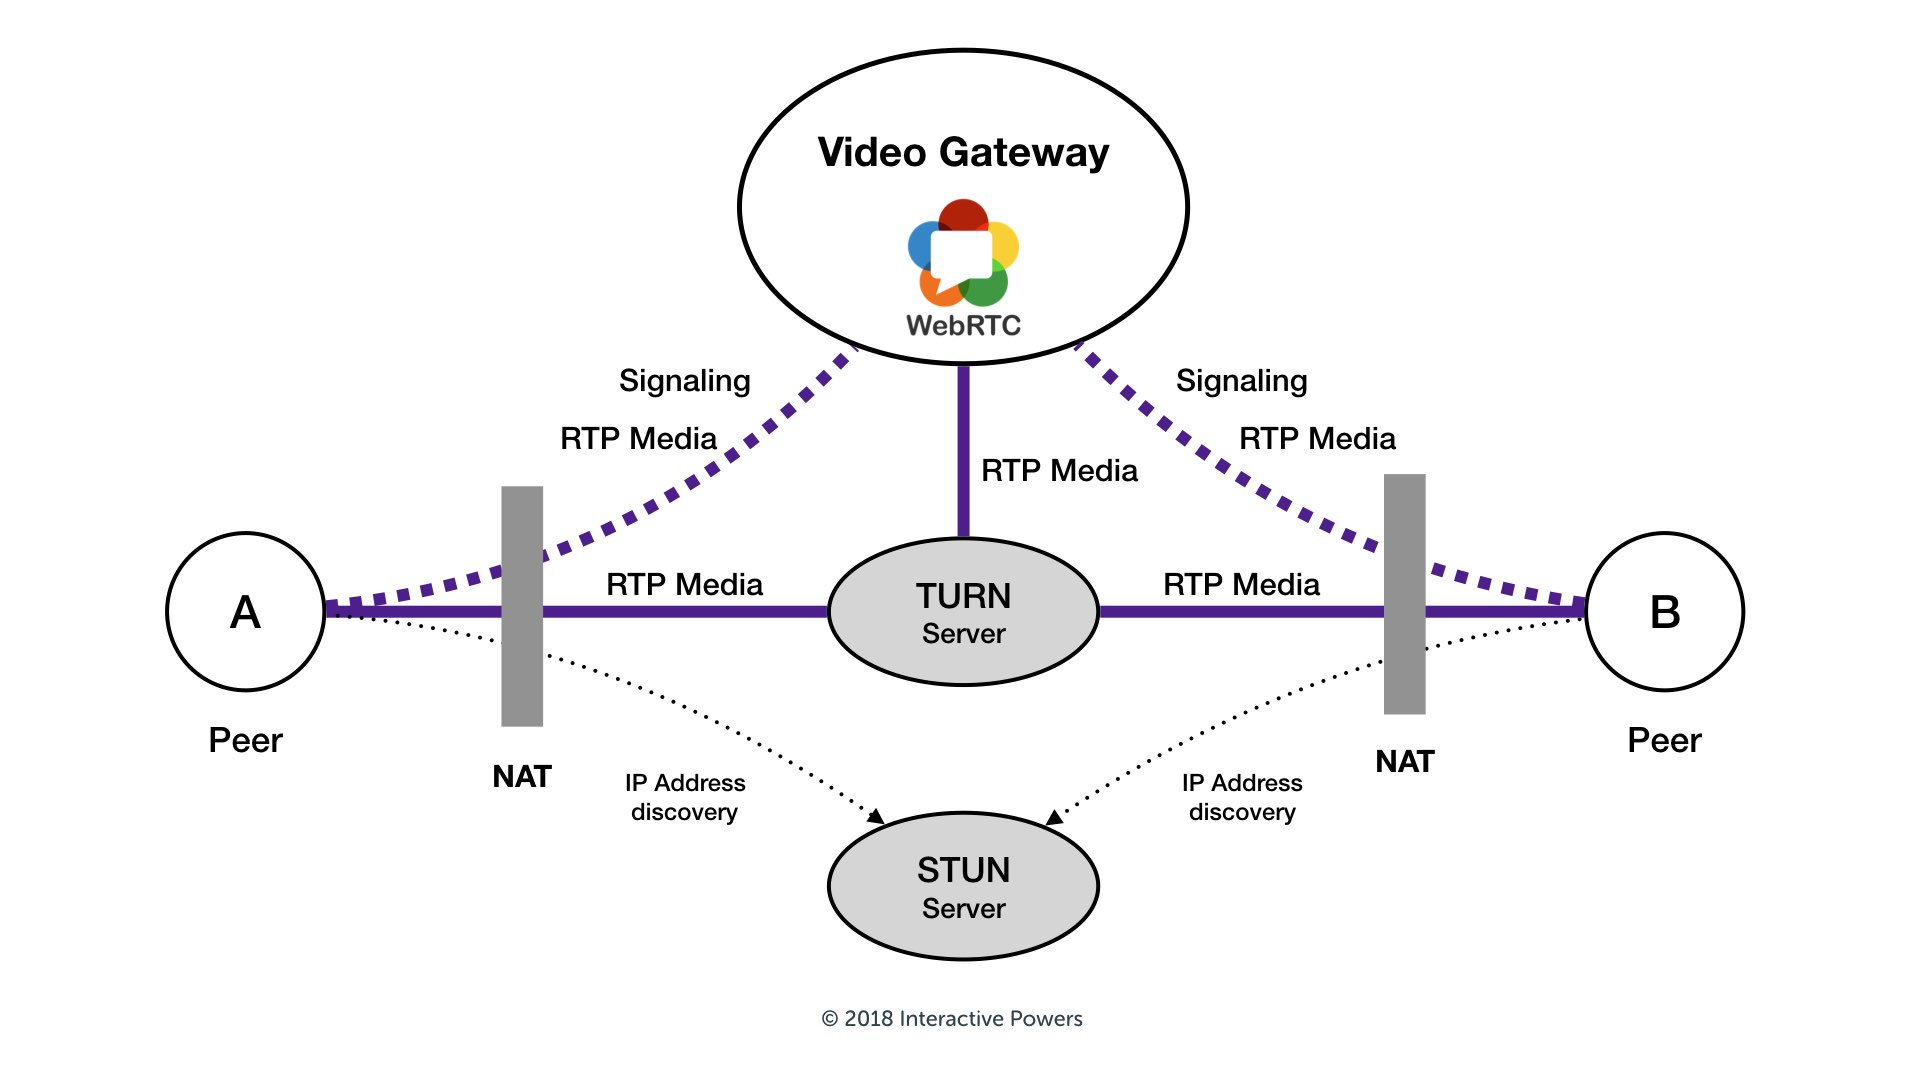
\includegraphics[width=\linewidth]{document/chapters/chapter_7/images/webrtc.jpeg}
    \caption{WebRTC - STUN and TURN servers \cite{stun_and_turn_servers}}
    \label{fig:webrtc}
\end{figure}

Free STUN and TURN servers (used by this prototype) are available thanks to the \textbf{\href{https://www.metered.ca/tools/openrelay/}{Open Relay}} initiative.

\subsection{Interconnected Mobile Client}
TODO

\begin{figure}[!ht]
    \centering
    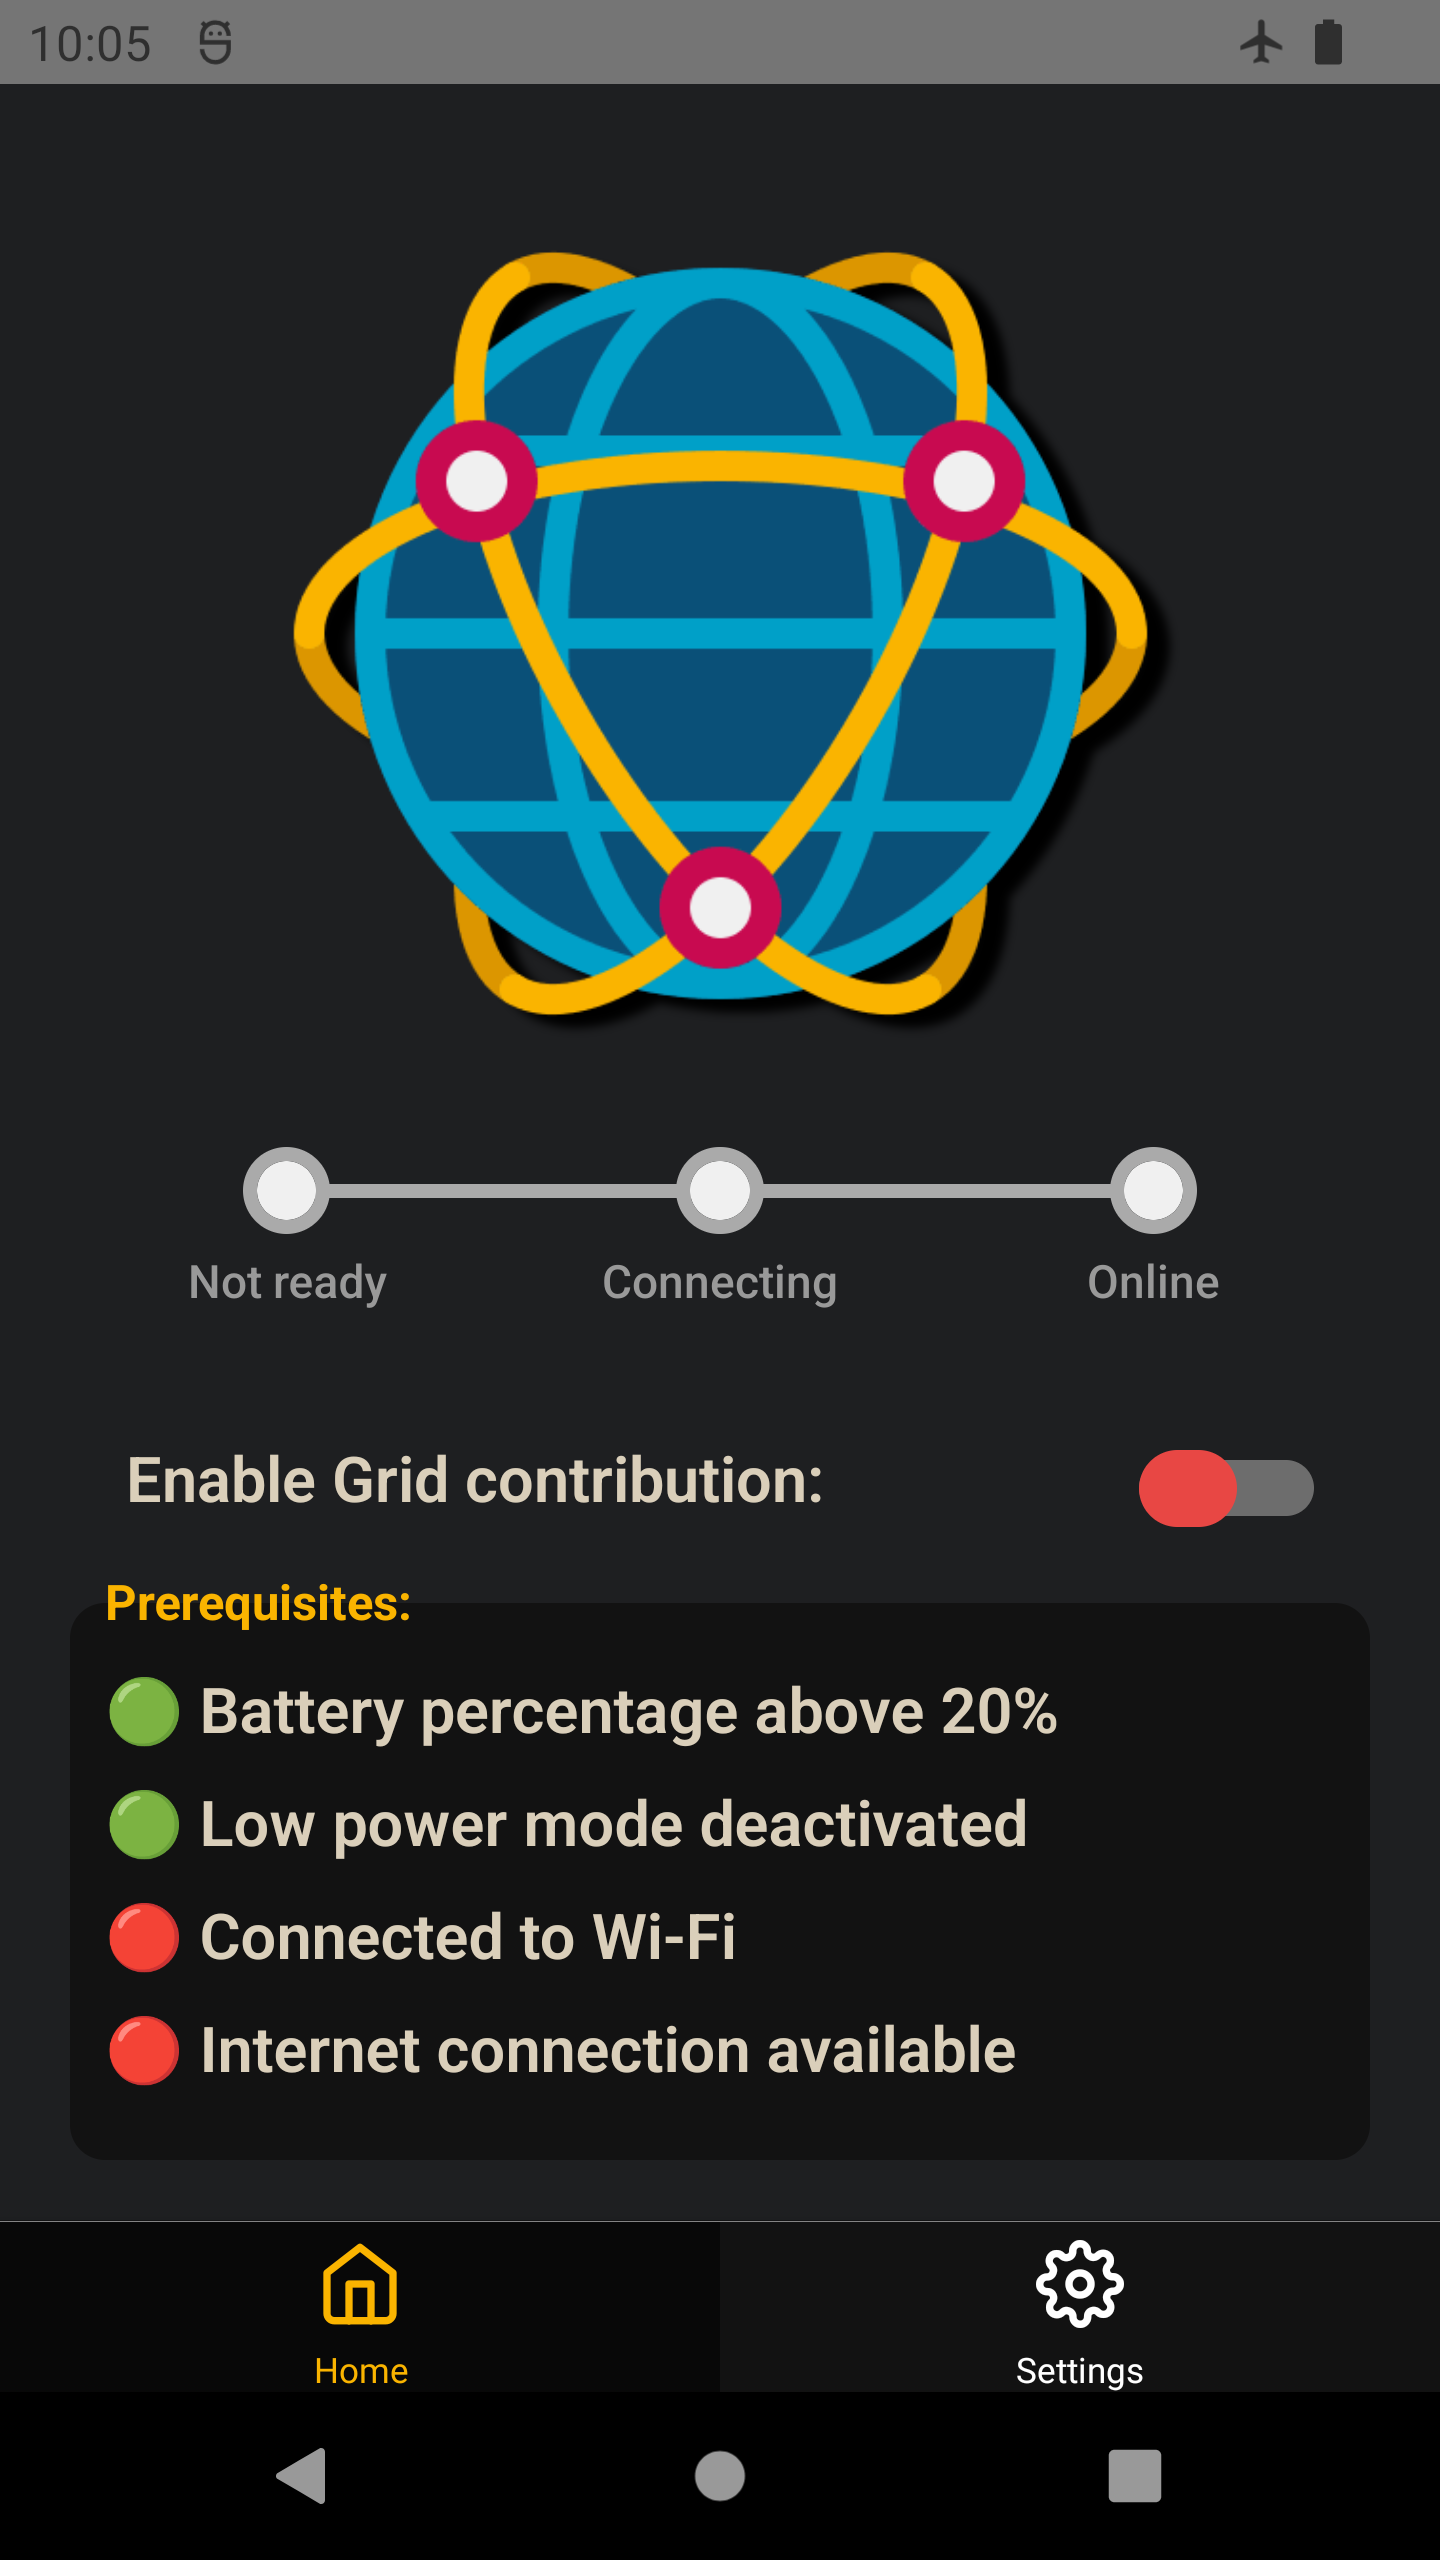
\includegraphics[scale=0.15]{document/chapters/chapter_7/images/interconnected_mobile_home.png}
    \caption{Interconnected Mobile Client}
    \label{fig:interconnected_mobile_home}
\end{figure}

\begin{figure}[!ht]
    \centering
    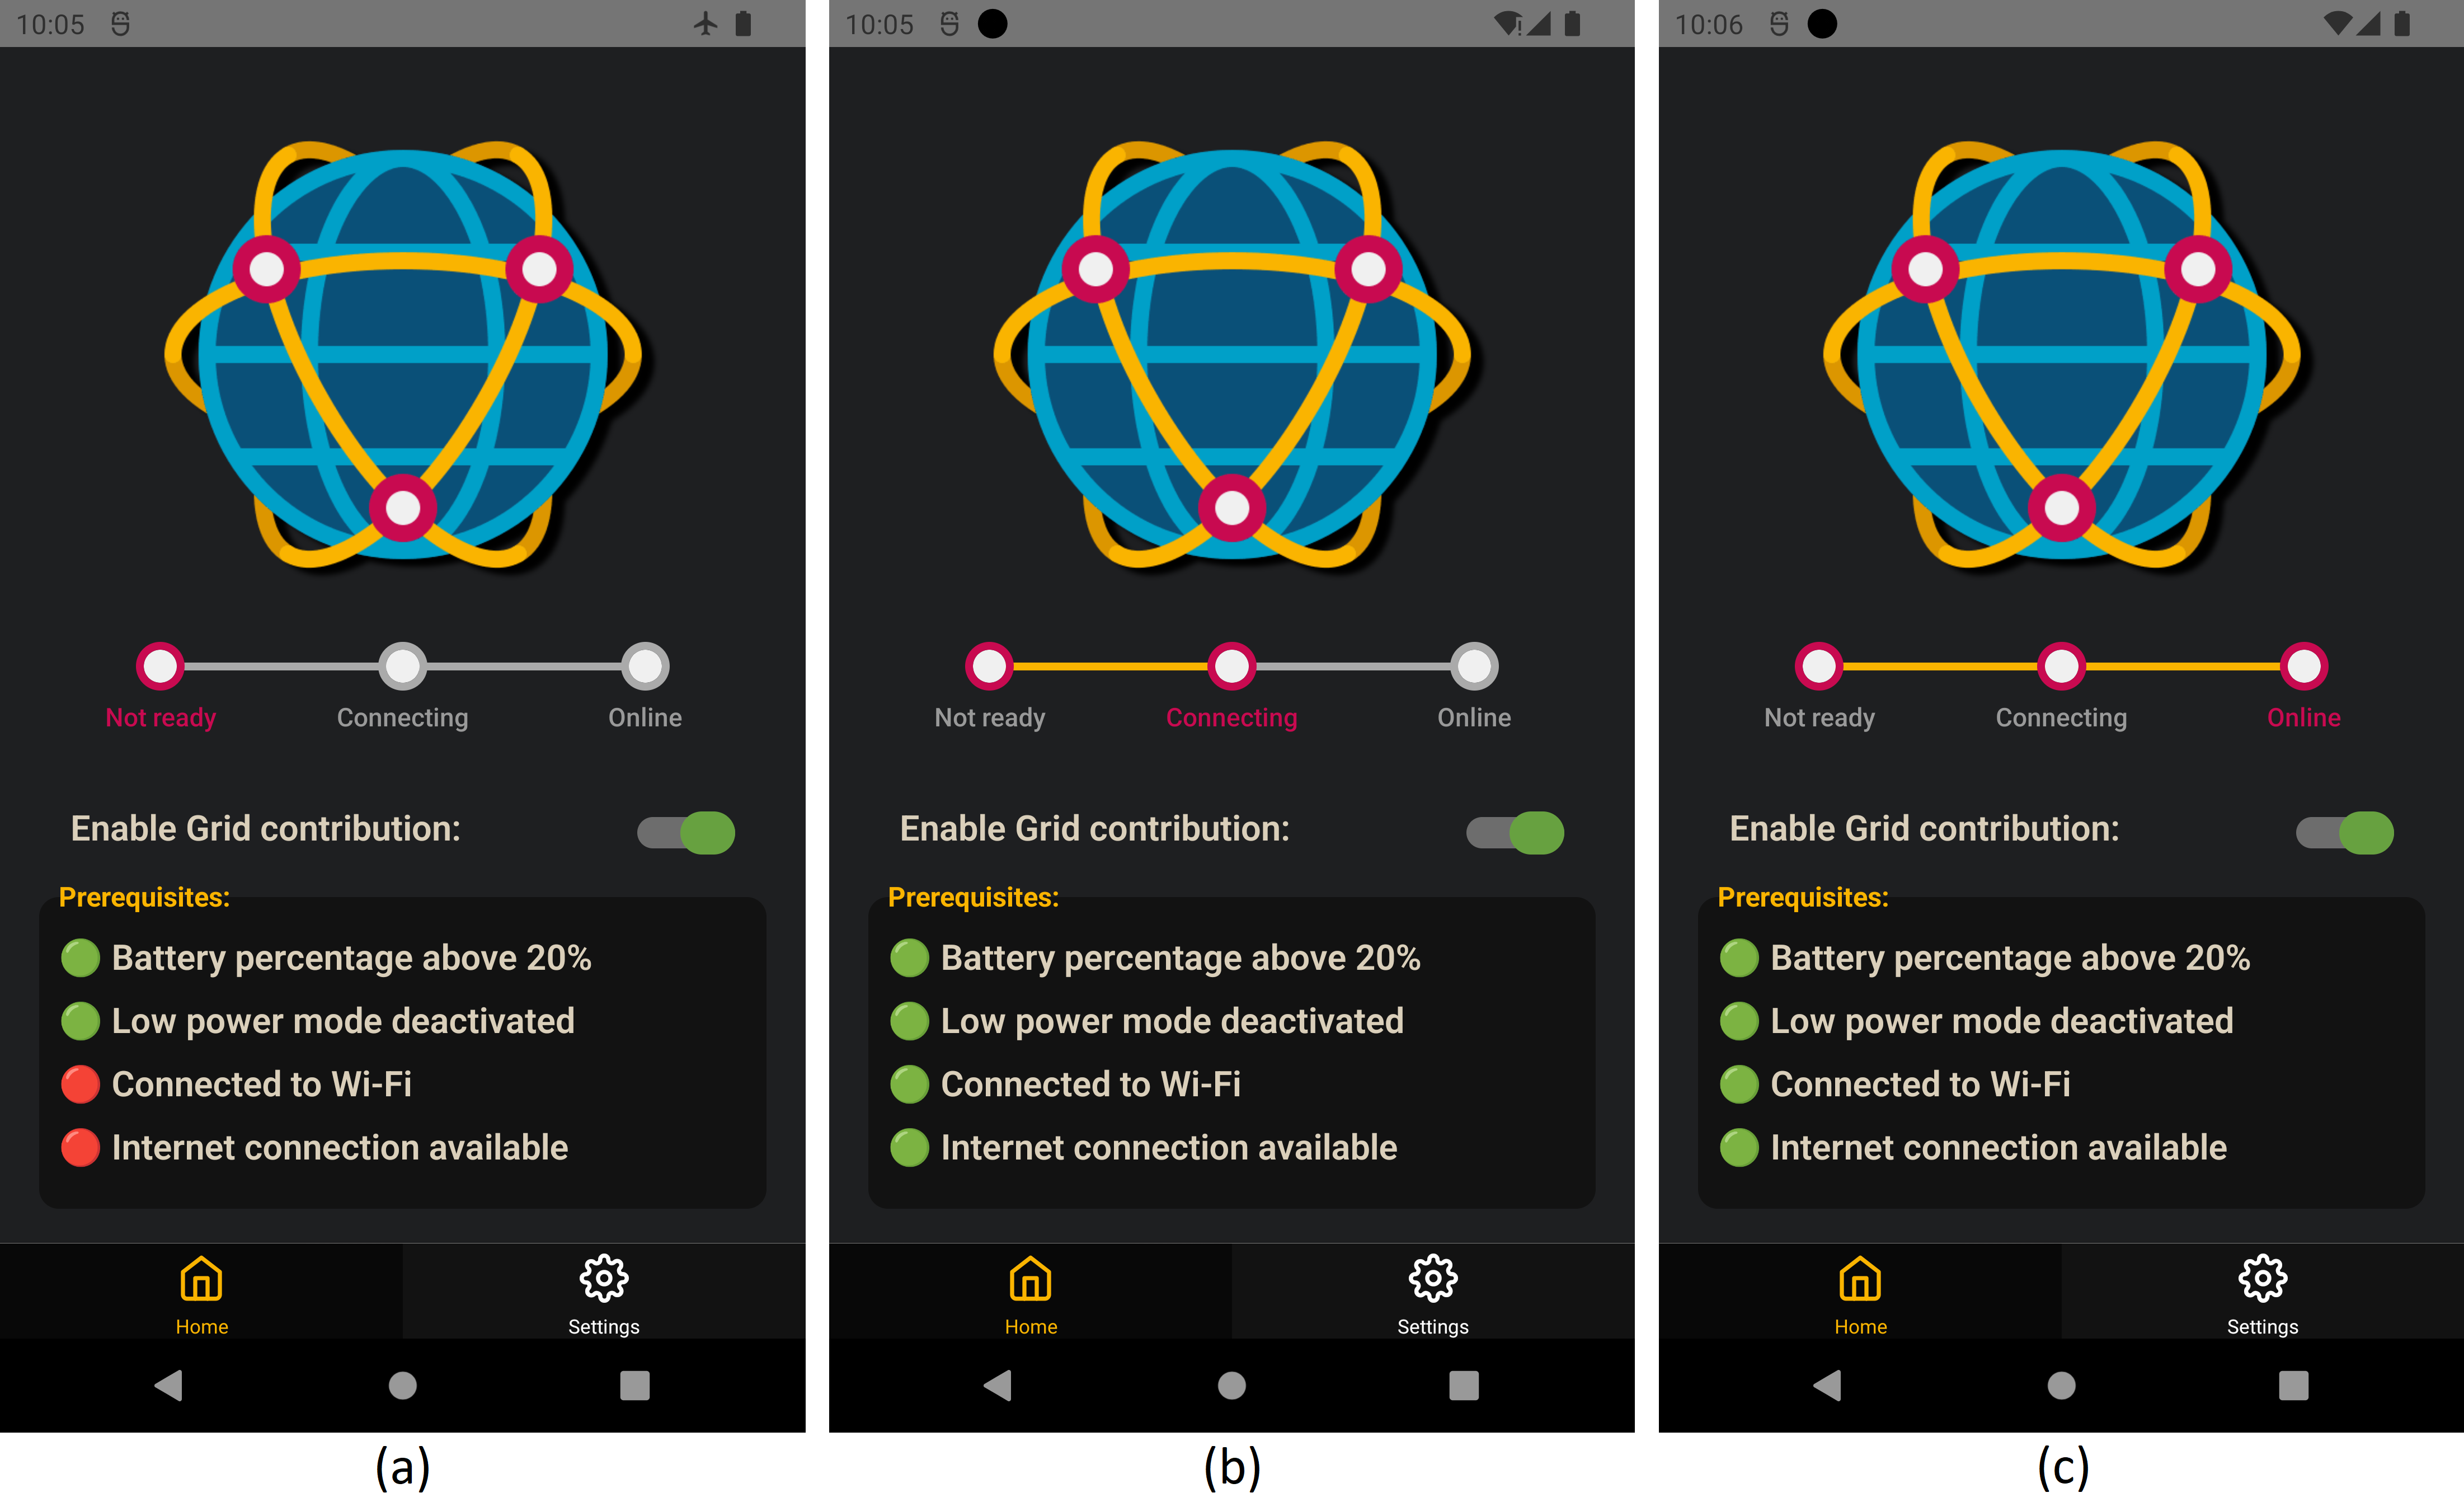
\includegraphics[width=\linewidth]{document/chapters/chapter_7/images/interconnected_mobile_connection.png}
    \caption{Interconnected Mobile Client - Connection}
    \label{fig:interconnected_mobile_connection}
\end{figure}

\begin{figure}[!ht]
    \centering
    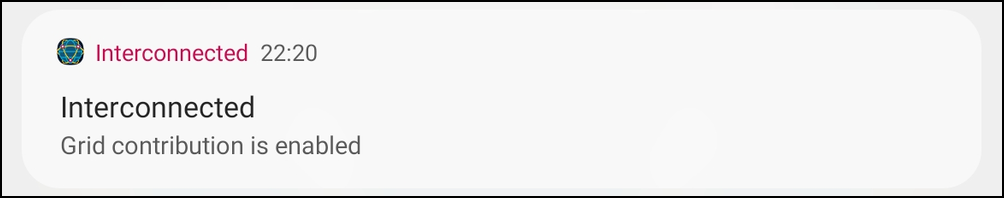
\includegraphics[scale=0.3]{document/chapters/chapter_7/images/notification_contribution.png}
    \caption{Interconnected Mobile Client - Grid contribution enabled notification}
    \label{fig:notification_contribution}
\end{figure}

\begin{figure}[!ht]
    \centering
    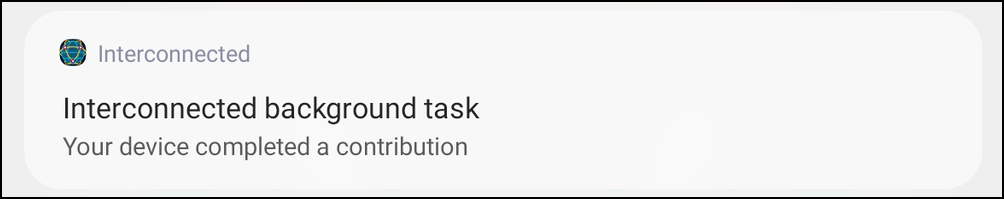
\includegraphics[scale=0.3]{document/chapters/chapter_7/images/notification_completed.png}
    \caption{Interconnected Mobile Client - Grid contribution completed notification}
    \label{fig:notification_completed}
\end{figure}

\subsection{Interconnected Desktop Client}
TODO

\begin{figure}[!ht]
    \centering
    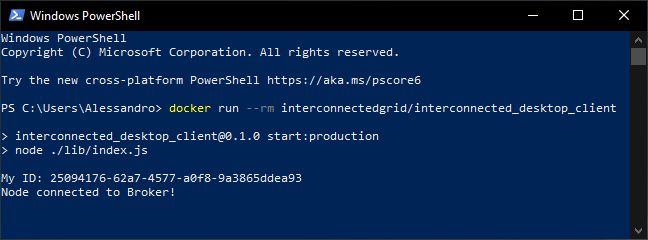
\includegraphics[scale=0.8]{document/chapters/chapter_7/images/interconnected_desktop.png}
    \caption{Interconnected Desktop Client - Docker image run on a container}
    \label{fig:interconnected_desktop}
\end{figure}

\subsection{Invoking Endpoint Prototype}
TODO